\documentclass{beamer}
\usepackage[utf8]{inputenc}
\usepackage[francais]{babel}
\usepackage[T1]{fontenc}
\usepackage[export]{adjustbox}
\newcommand\Fontvi{\fontsize{8}{7.2}\selectfont}

\usetheme{Warsaw}

\addtobeamertemplate{navigation symbols}{}{%
    \usebeamerfont{footline}%
    \usebeamercolor[fg]{footline}%
    \hspace{1em}%
    \insertframenumber/\inserttotalframenumber
}

\begin{document}
\logo{%
	\makebox[0.95\paperwidth]{%
		
\includegraphics[width=2.5cm,keepaspectratio]{images/hepia.jpg}%
		\hfill%
		
\includegraphics[width=2.5cm,keepaspectratio]{images/hesso.jpg}%
	}%
}

\title{MyLab2 GB}
\subtitle{Émulateur de Gameboy sur MyLab2}
\author{Orphée Antoniadis}
\institute{Projet de semestre - Prof. Fabien Vannel - Hepia ITI 3\up{ème} année}
\date{\today}

\begin{frame}
\titlepage
\end{frame}

\begin{frame}
	\setcounter{tocdepth}{1}
	\tableofcontents
\end{frame}

%%%%%%%%%%%%%%%%%%%%%%%%%%%%%%%%%%%%%%%%%%%%%%%%%%%%%%%%%%%%%%%%%%
%%%%%%%%%%%%%%%%%%%%%%%%%%%%%%%%%%%%%%%%%%%%%%%%%%%%%%%%%%%%%%%%%%

\section{Introduction}
\subsection{Objectifs du projet}
\begin{frame}
	\frametitle{\secname}
	\framesubtitle{\subsecname}
	\begin{itemize}
		\item Comprendre le fonctionnement d'une Gameboy
    \item Comprendre la logique derrière un émulateur
    \item Faire un émulateur de Gameboy sur la carte MyLab2
		\item Analyser les contraintes du projet
	\end{itemize}
\end{frame}

%%%%%%%%%%%%%%%%%%%%%%%%%%%%%%%%%%%%%%%%%%%%%%%%%%%%%%%%%%%%%%%%%%

\subsection{Méthode}
\begin{frame}
	\frametitle{\secname}
	\framesubtitle{\subsecname}
	\begin{itemize}
		\item Recherches
		\item Implémentation de l'émulateur
    \item Tests avec la carte MyLab2
	\end{itemize}
\end{frame}

%%%%%%%%%%%%%%%%%%%%%%%%%%%%%%%%%%%%%%%%%%%%%%%%%%%%%%%%%%%%%%%%%%
%%%%%%%%%%%%%%%%%%%%%%%%%%%%%%%%%%%%%%%%%%%%%%%%%%%%%%%%%%%%%%%%%%

\section{MyLab2}
\subsection{Introduction}
\begin{frame}
	\frametitle{\secname}
  \framesubtitle{\subsecname}
  \begin{columns}[T]
		\begin{column}{.30\textwidth}
			\begin{figure}
				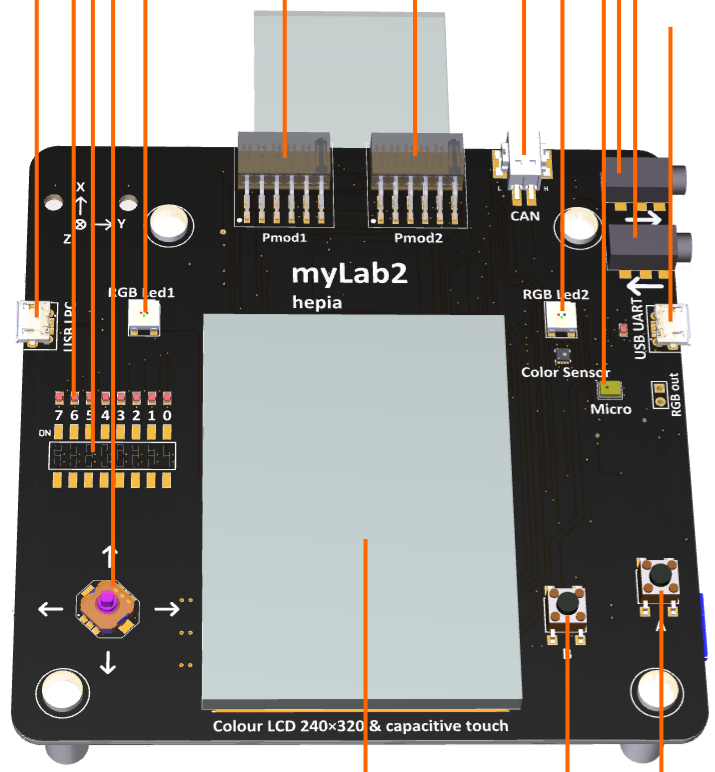
\includegraphics[width=1\textwidth]{images/mylab2.png}
			\end{figure}
		\end{column}
		\begin{column}{.70\textwidth}
			\begin{itemize}
				\item Carte d'extension pour LPC1769 et LPC4337
				\item Développée au LSN à hepia
				\item Jusqu'à 120MHz de fréquence d'horloge
        \item 512kB de mémoire flash
        \item 64kB de SRAM
			\end{itemize}
		\end{column}
	\end{columns}
\end{frame}

%%%%%%%%%%%%%%%%%%%%%%%%%%%%%%%%%%%%%%%%%%%%%%%%%%%%%%%%%%%%%%%%%%

\subsection{Périphériques utilisés}
\begin{frame}
	\frametitle{\secname}
  \framesubtitle{\subsecname}
  \begin{center}
    \begin{figure}
      \only<1>{
        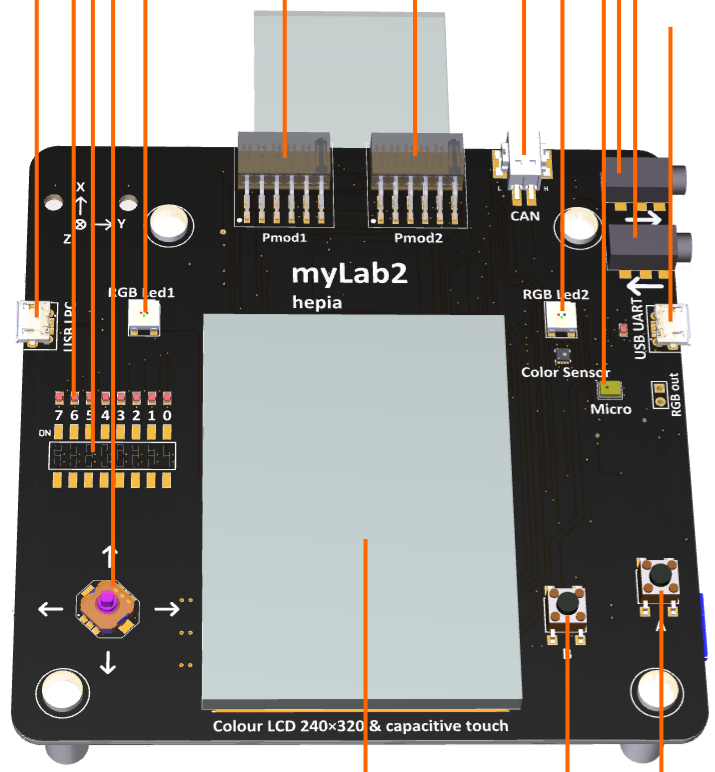
\includegraphics[width=.35\textwidth]{images/mylab2.png}
        \caption{MyLab2}
      }
      \only<2>{
        \includegraphics[width=.35\textwidth]{images/mylab2_lcd.png}
        \caption{Ecran LCD / Dalle tactile}
      }
      \only<3>{
        \includegraphics[width=.35\textwidth]{images/mylab2_joypad.png}
        \caption{Joystick}
      }
      \only<4>{
        \includegraphics[width=.35\textwidth]{images/mylab2_buttons.png}
        \caption{Boutons A et B}
      }
      \only<5>{
        \includegraphics[width=.35\textwidth]{images/mylab2_uart.png}
        \caption{UART}
      }
    \end{figure}
  \end{center}
\end{frame}

%%%%%%%%%%%%%%%%%%%%%%%%%%%%%%%%%%%%%%%%%%%%%%%%%%%%%%%%%%%%%%%%%%
%%%%%%%%%%%%%%%%%%%%%%%%%%%%%%%%%%%%%%%%%%%%%%%%%%%%%%%%%%%%%%%%%%

\section{Gameboy}
\subsection{Présentation}
\begin{frame}
	\frametitle{\secname}
  \framesubtitle{\subsecname}
  \begin{columns}[T]
		\begin{column}{.30\textwidth}
			\begin{figure}
				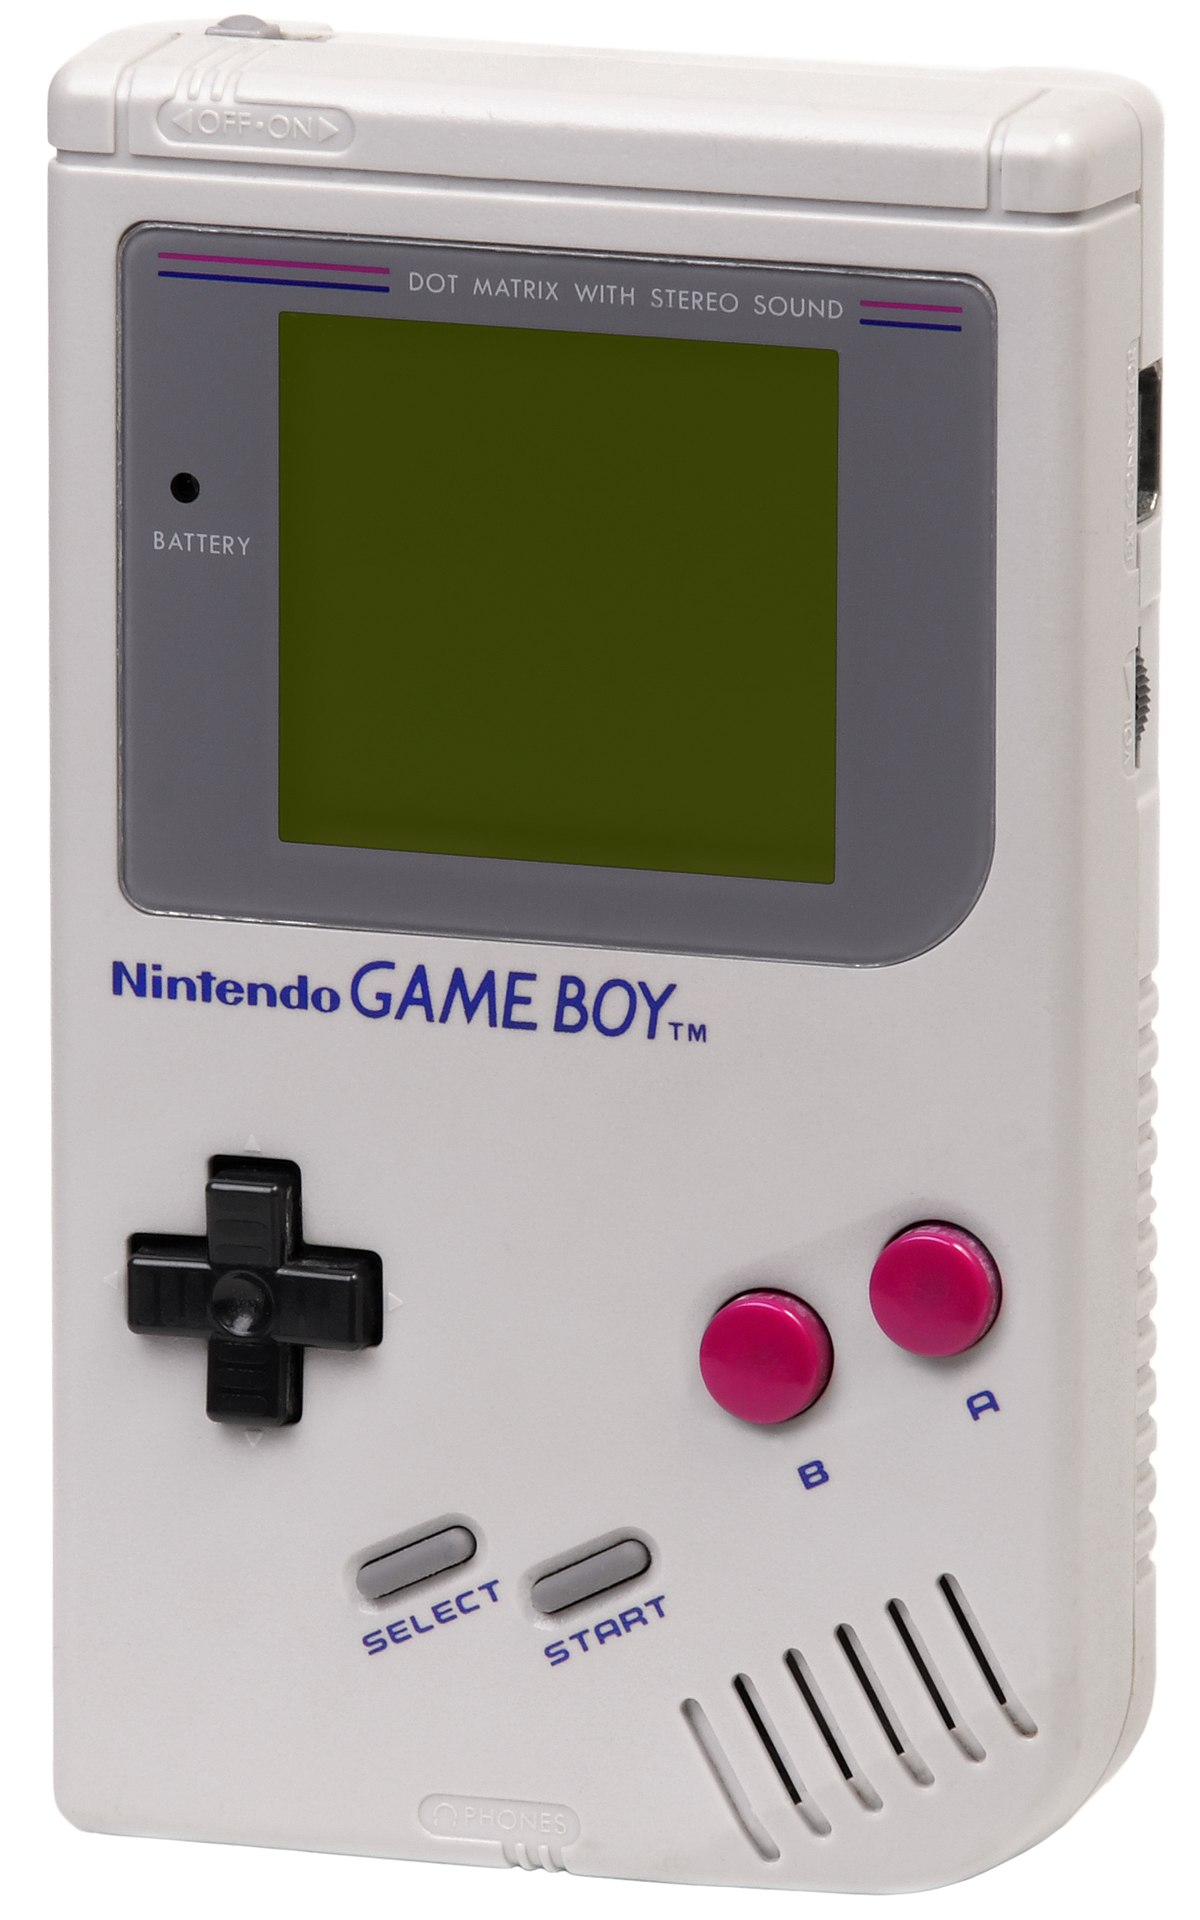
\includegraphics[width=.6\textwidth]{images/gameboy.jpg}
				\caption{Gameboy}
			\end{figure}
		\end{column}
		\begin{column}{.70\textwidth}
			\begin{itemize}
				\item Console de jeux vidéos portable
        \item Développée et fabriquée par Nintendo
				\item Mise en vente en 1989
      \end{itemize}
		\end{column}
	\end{columns}
\end{frame}

%%%%%%%%%%%%%%%%%%%%%%%%%%%%%%%%%%%%%%%%%%%%%%%%%%%%%%%%%%%%%%%%%%

\subsection{Processeur}
\begin{frame}
	\frametitle{\secname}
  \framesubtitle{\subsecname}
  \begin{columns}[T]
		\begin{column}{.30\textwidth}
			\begin{figure}
				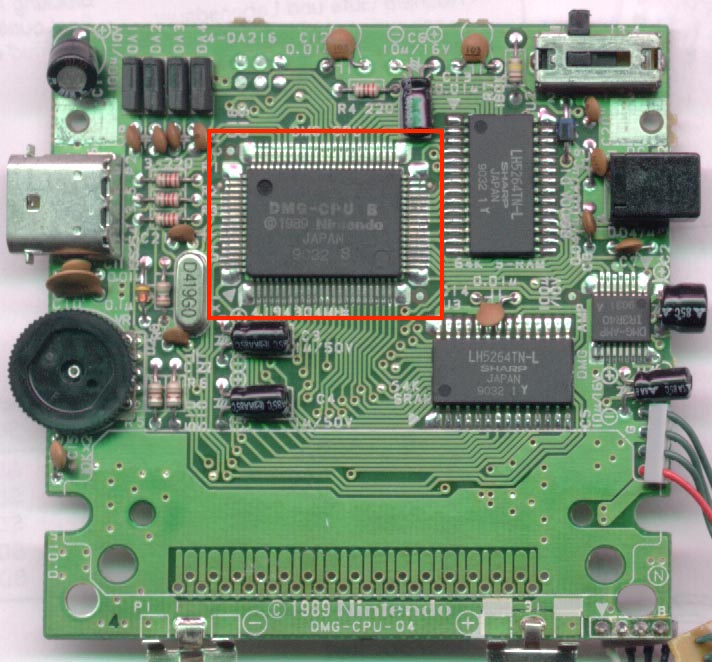
\includegraphics[width=1\textwidth]{images/cpu.jpg}
				\caption{CPU}
			\end{figure}
		\end{column}
		\begin{column}{.70\textwidth}
      \begin{itemize}
        \item Processeur 8 bits ($256*2$ instructions)
        \item 6 registres de 16 bits
      \end{itemize}
      \begin{center}
        \scalebox{0.8}{
          \begin{tabular}{| c | c | c |}
            \hline
            AF & A : registre & F : flags \\ \hline
            BC & B : registre & C : registre \\ \hline
            DE & D : registre & E : registre \\ \hline
            HL & H : registre & L : registre \\ \hline
            SP & \multicolumn{2}{|c|}{Stack pointer} \\ \hline
            PC & \multicolumn{2}{|c|}{Program counter} \\ \hline
          \end{tabular}
        }
      \end{center}
      \begin{itemize}
        \item Cadencé à 4,19MHz
        \item Méchanismes d'interruptions
      \end{itemize}
		\end{column}
	\end{columns}
\end{frame}

%%%%%%%%%%%%%%%%%%%%%%%%%%%%%%%%%%%%%%%%%%%%%%%%%%%%%%%%%%%%%%%%%%

\subsection{Mémoire}
\begin{frame}
	\frametitle{\secname}
  \framesubtitle{\subsecname}
  \begin{center}
    \scalebox{0.7}{
      \begin{tabular}{| c | c | c |}
        \hline
        Adresses & Nom & Description \\ \hline
        0000h – 3FFFh & ROM0 & ROM non-échangeable \\ \hline
        4000h – 7FFFh & ROMX & ROM échangeable \\ \hline
        8000h – 9FFFh & VRAM & Video RAM \\ \hline
        A000h – BFFFh & SRAM & RAM externe \\ \hline
        C000h – CFFFh & WRAM0 & Work RAM \\ \hline
        D000h – DFFFh & WRAMX & Work RAM échangeable \\ \hline
        E000h – FDFFh & ECHO & Echo de la WRAM \\ \hline
        FE00h – FE9Fh & OAM & Sprites \\ \hline
        FEA0h – FEFFh & UNUSED & - \\ \hline
        FF00h – FF7Fh & I/O Registers & - \\ \hline
        FF80h – FFFEh & HRAM & RAM interne du CPU \\ \hline
        FFFFh & IE Register & Registre d'activation des interruptions \\ \hline
      \end{tabular}
    }
  \end{center}
\end{frame}

%%%%%%%%%%%%%%%%%%%%%%%%%%%%%%%%%%%%%%%%%%%%%%%%%%%%%%%%%%%%%%%%%%

\subsection{Écran}
\begin{frame}
	\frametitle{\secname}
  \framesubtitle{\subsecname}
  \begin{columns}[T]
		\begin{column}{.30\textwidth}
			\begin{figure}
				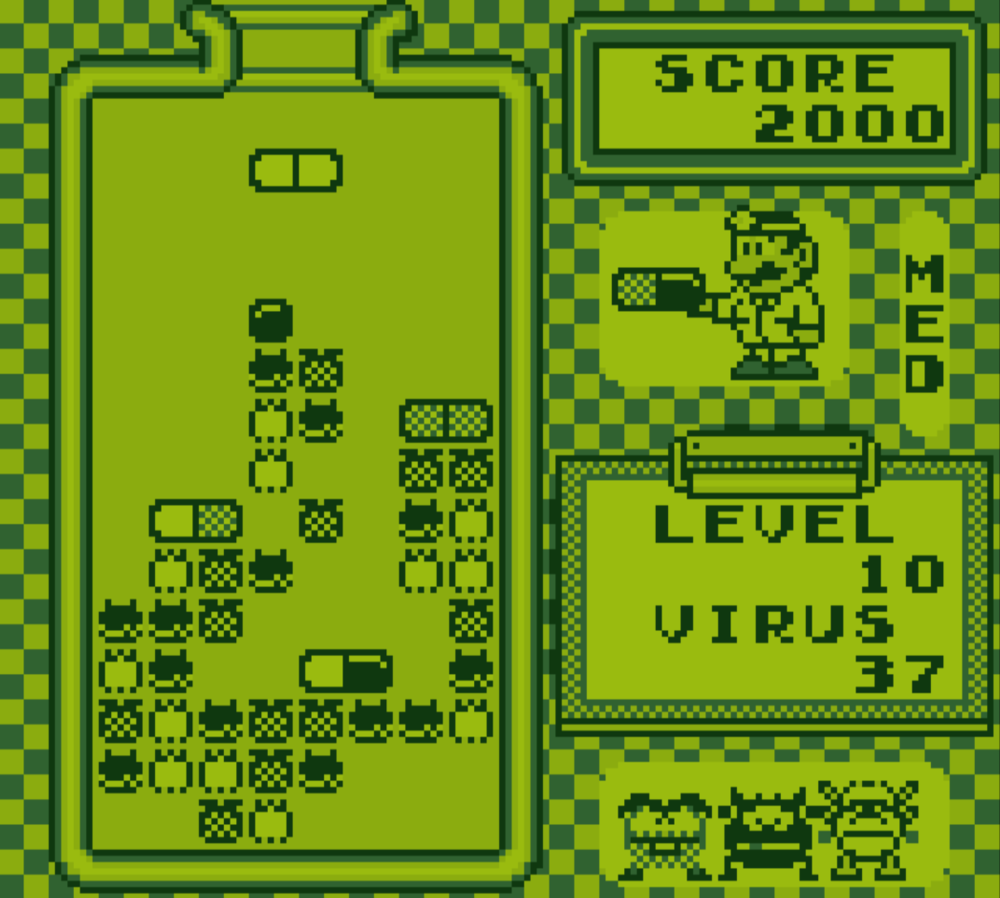
\includegraphics[width=1\textwidth]{images/screen.png}
				\caption{Écran}
			\end{figure}
		\end{column}
		\begin{column}{.70\textwidth}
      \begin{itemize}
        \item 2,6 pouces
        \item 160x144px
        \item 4 nuances de gris
        \item 3 types d'éléments :
        \begin{itemize}
          \item Background
          \item Window
          \item Sprites
        \end{itemize}
      \end{itemize}
		\end{column}
	\end{columns}
\end{frame}

%%%%%%%%%%%%%%%%%%%%%%%%%%%%%%%%%%%%%%%%%%%%%%%%%%%%%%%%%%%%%%%%%%

\subsection{Autres}
\begin{frame}
	\frametitle{\secname}
  \framesubtitle{\subsecname}
  \begin{itemize}
    \item Timer
    \item DMA
    \item Boutons A, B, START et SELECT
    \item Croix directionnelle
    \item Son
    \item Communication série
  \end{itemize}
\end{frame}

%%%%%%%%%%%%%%%%%%%%%%%%%%%%%%%%%%%%%%%%%%%%%%%%%%%%%%%%%%%%%%%%%%
%%%%%%%%%%%%%%%%%%%%%%%%%%%%%%%%%%%%%%%%%%%%%%%%%%%%%%%%%%%%%%%%%%

\section{Emulateur}
\subsection{Diagramme}
\begin{frame}
	\frametitle{\secname}
  \framesubtitle{\subsecname}
  \begin{center}
    \begin{figure}
      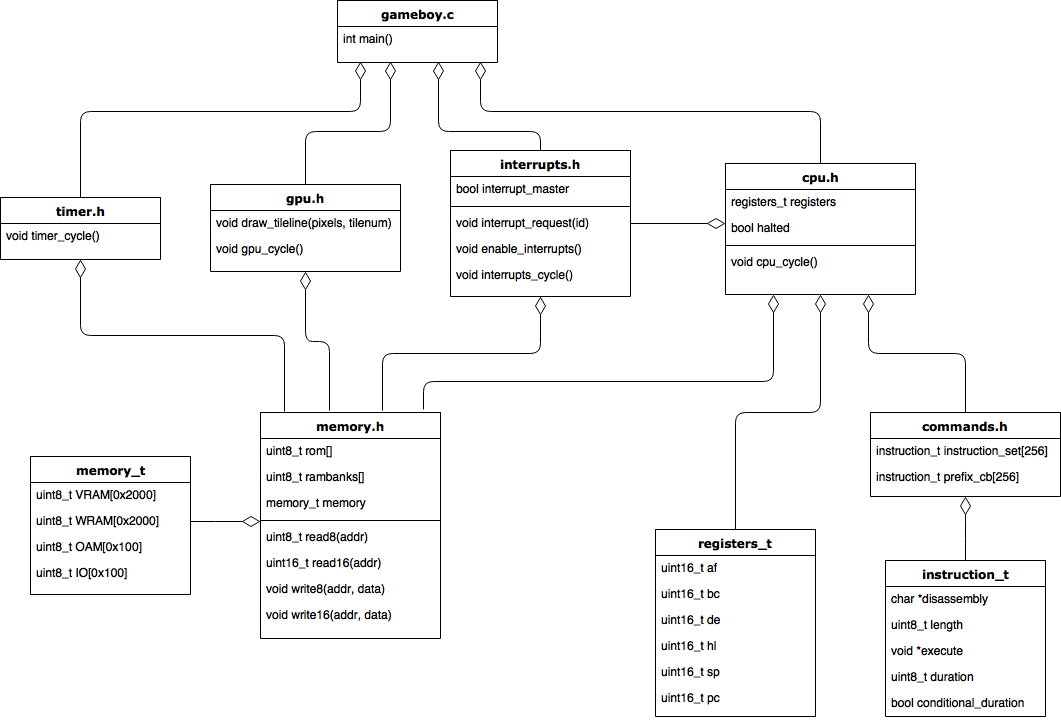
\includegraphics[width=.50\textwidth]{images/class_diag.png}
    \end{figure}
  \end{center}
\end{frame}

%%%%%%%%%%%%%%%%%%%%%%%%%%%%%%%%%%%%%%%%%%%%%%%%%%%%%%%%%%%%%%%%%%

\subsection{Debug}
\begin{frame}
	\frametitle{\secname}
  \framesubtitle{\subsecname}
  \begin{columns}[T]
		\begin{column}{.30\textwidth}
			\begin{figure}
				\includegraphics[width=1\textwidth]{images/blargg.png}
			\end{figure}
		\end{column}
		\begin{column}{.70\textwidth}
      Problèmes rencontrés:
      \begin{itemize}
        \item Emulateur trop lent pour tester l'affichage
        \item Beaucoup d'informations trouvées
        \item Problème de fiabilité des sources
      \end{itemize}
      Solutions:
      \begin{itemize}
        \item Utilisation de la SDL pour déboguer l'affichage
        \item Tests unitaires (Blargg et Mooneye)
      \end{itemize}
		\end{column}
	\end{columns}
\end{frame}

%%%%%%%%%%%%%%%%%%%%%%%%%%%%%%%%%%%%%%%%%%%%%%%%%%%%%%%%%%%%%%%%%%

\subsection{Features}
\begin{frame}
	\frametitle{\secname}
  \framesubtitle{\subsecname}
  \begin{columns}[T]
		\begin{column}{.50\textwidth}
      \begin{itemize}
        \item Affichage fonctionnel
        \item Jouable
      \end{itemize}
		\end{column}
    \begin{column}{.50\textwidth}
			\begin{figure}
				\includegraphics[width=1\textwidth]{images/features1.png}
			\end{figure}
		\end{column}
	\end{columns}
\end{frame}
\begin{frame}
	\frametitle{\secname}
  \framesubtitle{\subsecname}
  \begin{columns}[T]
		\begin{column}{.50\textwidth}
      \begin{itemize}
        \item Affichage fonctionnel
        \item Jouable
        \item Multiplateforme
      \end{itemize}
		\end{column}
    \begin{column}{.50\textwidth}
			\begin{figure}
				\includegraphics[width=1\textwidth]{images/features2.png}
			\end{figure}
		\end{column}
	\end{columns}
\end{frame}
\begin{frame}
	\frametitle{\secname}
  \framesubtitle{\subsecname}
  \begin{columns}[T]
		\begin{column}{.50\textwidth}
      \begin{itemize}
        \item Affichage fonctionnel
        \item Jouable
        \item Multiplateforme
        \item Logs
      \end{itemize}
		\end{column}
    \begin{column}{.50\textwidth}
			\begin{figure}
				\includegraphics[width=1\textwidth]{images/features3.png}
			\end{figure}
		\end{column}
	\end{columns}
\end{frame}
\begin{frame}
	\frametitle{\secname}
  \framesubtitle{\subsecname}
  \begin{columns}[T]
		\begin{column}{.50\textwidth}
      \begin{itemize}
        \item Affichage fonctionnel
        \item Jouable
        \item Multiplateforme
        \item Logs
        \item Open source
      \end{itemize}
		\end{column}
    \begin{column}{.50\textwidth}
			\begin{figure}
				\includegraphics[width=1\textwidth]{images/features4.png}
			\end{figure}
		\end{column}
	\end{columns}
\end{frame}
\begin{frame}
	\frametitle{\secname}
  \framesubtitle{\subsecname}
  \begin{columns}[T]
		\begin{column}{.50\textwidth}
      \begin{itemize}
        \item Affichage fonctionnel
        \item Jouable
        \item Multiplateforme
        \item Logs
        \item Open source
        \item Jusqu'à 12 FPS !
      \end{itemize}
		\end{column}
    \begin{column}{.50\textwidth}
			\begin{figure}
				\includegraphics[width=1\textwidth]{images/features4.png}
			\end{figure}
		\end{column}
	\end{columns}
\end{frame}

%%%%%%%%%%%%%%%%%%%%%%%%%%%%%%%%%%%%%%%%%%%%%%%%%%%%%%%%%%%%%%%%%%
%%%%%%%%%%%%%%%%%%%%%%%%%%%%%%%%%%%%%%%%%%%%%%%%%%%%%%%%%%%%%%%%%%

\section{Résultats et améliorations}
\begin{frame}
	\frametitle{\secname}
  \begin{columns}[T]
		\begin{column}{.40\textwidth}
			\begin{figure}
				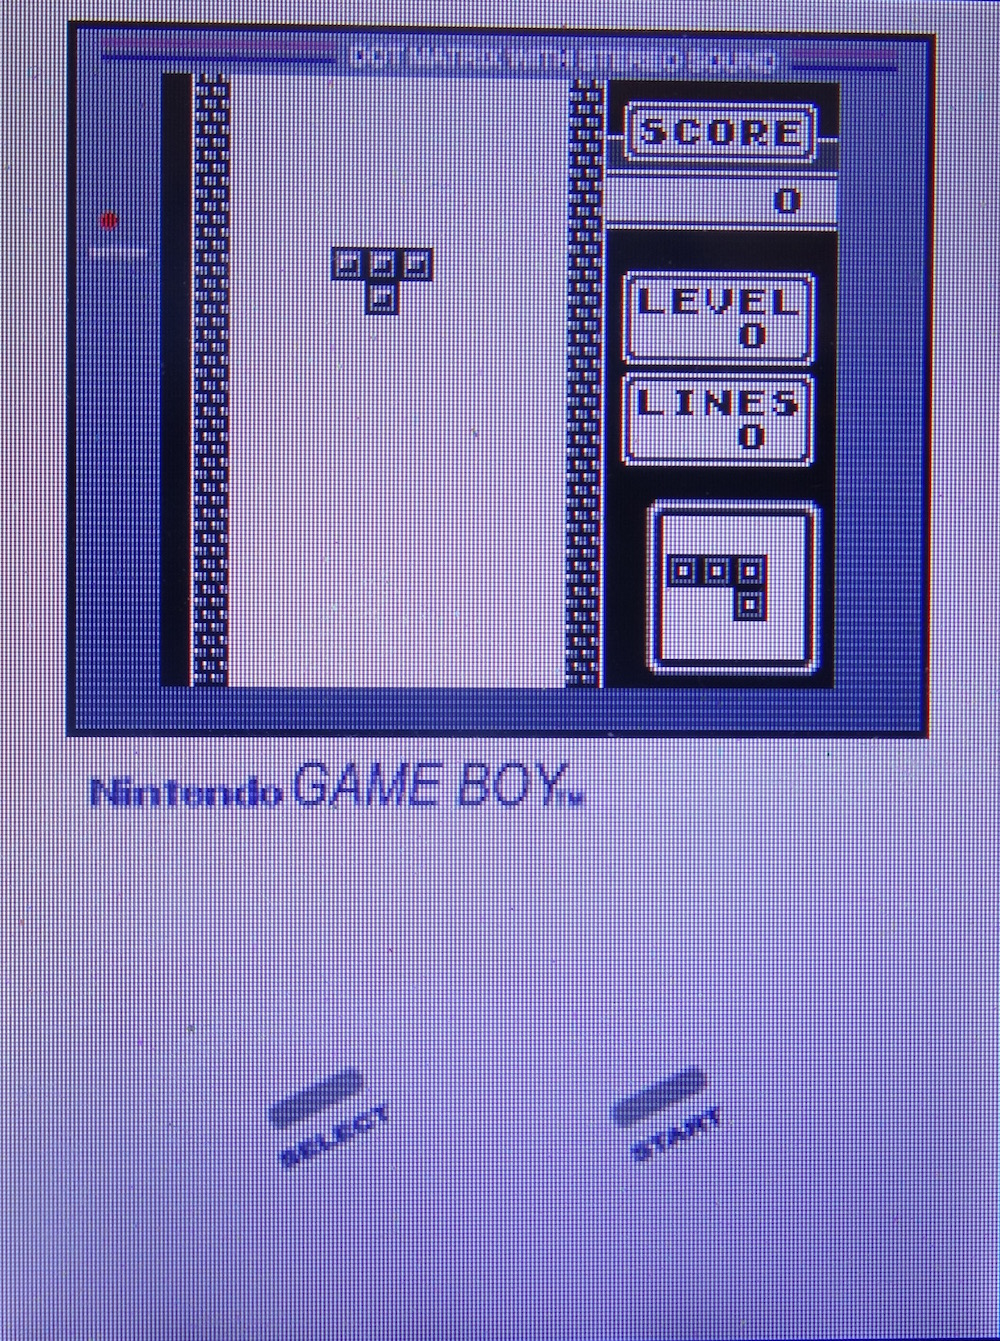
\includegraphics[width=.75\textwidth]{images/mylab2gb.jpg}
			\end{figure}
		\end{column}
		\begin{column}{.70\textwidth}
      Résultats:
      \begin{itemize}
        \item Emulateur fonctionnel mais lent
        \item Compréhension des limites du LPC1769
      \end{itemize}
      Possibles améliorations:
      \begin{itemize}
        \item Ajouter toutes les fonctionnalités de la Gameboy
        \item Porter sur le LPC4337
        \item Emuler le processeur de la Gameboy sur FPGA
      \end{itemize}
		\end{column}
	\end{columns}
\end{frame}

\end{document}
